\documentclass{beamer}

%%----Packages
\usepackage{fontspec}
% used to set font for the latex document.

\usepackage[CJKchecksingle]{xeCJK}
% using CJK to manage Chinese, need fontsec.
\setCJKmainfont[BoldFont={方正黑体简体}, ItalicFont={方正楷体简体}]{方正大标宋简体}
\setCJKsansfont{方正黑体简体}
\setCJKmonofont{方正中等线简体}

\usepackage{textcomp}    % provide symbols.

\usepackage{graphicx}
\graphicspath{{pic/}}
\usepackage{tikz}

\usetheme{PKULabMeeting}


\title{一个 PKULabMeeting 模版}
\author{小狼}
\institute{Peking University}    % provide the information of institute. 
\date{\today}
\logo{
\includegraphics[height=0.6\textheight]{pku.png}}
\titlepagelogo{
\includegraphics[width=0.3\textwidth]{pku.png}}
\titlepagebackground{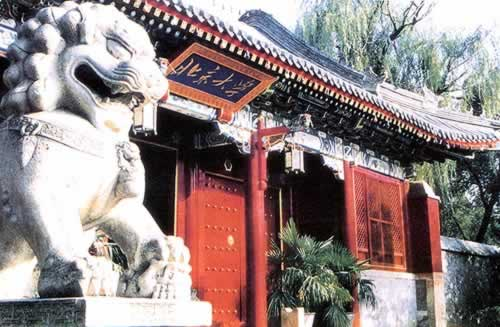
\includegraphics[height=7cm]{gate.jpg}}
\department{School of Life Sciences}
\backgroundlogo{
\includegraphics[height=4cm]{cloud.png}}


\begin{document}

%-*-coding:utf-8-*-
%%%%%%%%%%%%%%%%%%%%%%%%%%%%%%%%%%%%%%%%%%%%%%%%%%%%%%%%%%%%%%%%%%%%%%%%%%%%%%%%
%% Name:   Work Report                                                        %%
%% Author: Wolfson                                                            %%
%% Date:   2017-02-07                                                         %%
%% Discription:                                                               %%
%%%%%%%%%%%%%%%%%%%%%%%%%%%%%%%%%%%%%%%%%%%%%%%%%%%%%%%%%%%%%%%%%%%%%%%%%%%%%%%%


\begin{frame}
  \maketitle
\end{frame}

\section*{Contents}

\begin{frame}{Contents}
  \tableofcontents
\end{frame}

%% ------------------

\thanksframe{Thanks!}

%% -----------------------------------------------------------------------------
\appendix
%{{{ Appendix

%}}}


%%%%%%%%%%%%%%%%%%%%%%%%%%%%%%%%%%%%%%%%%%%%%%%%%%%%%%%%%%%%%%%%%%%%%%%%%%%%%%%%
\endinput

 
\end{document}
